
\section{ODFs}


\subsection*{ODFs in MTEX}

% \begin{frame}
% \begin{tikzpicture}[every concept/.style={font=\small,minimum
% size=0pt,concept color=blue!10}]

% \tikzstyle{root concept}+=[text width=2cm]
% \tikzstyle{level 1 concept}+=[text width=1cm]

% \path[mindmap] node[concept] {Computer Science}
% child[concept] {node[concept] {laber}};
% \end{tikzpicture}
% \end{frame}


\begin{frame}[fragile]
  \frametitle{Orientation Density Functions in \MTEX}


 \begin{tikzpicture}[scale=0.85,every concept/.style={font=\small,minimum size=0pt}]
  \definecolor{myblue}{HTML}{92dcec}
  \tikzstyle{every annotation}=[fill=white, font=\sf]
  \tikzstyle{root concept}+=[text width=2cm]
  \tikzstyle{level 1 concept}+=[text width=1.3cm]

  \path[mindmap,concept color=orange!80!]
  node[concept](data) at (-7,0) {\bf Data}
  child[grow = 45, concept color=orange!50]
  { node(ebsd) [concept](ebsd2) {EBSD \\
      Data} }
  child[grow = -45, concept color=orange!50]
  { node[concept](pf) {Pole Figure\\Data}};

  \path[mindmap,concept color=blue!40!]
  node[concept](odf) {\bf ODF}
  child[grow = -45, concept color=blue!30!] { node [concept](zwei) {Fourier \\ ODF} }
  child[grow = -22.5, concept color=blue!30] { node[concept] {Bingham
      \\ ODF}}
  child[grow = 0, concept color=blue!30!] { node [concept](zwei) {Fibre \\ ODF} }
  child[grow = 22.5, concept color=blue!30] { node [concept] {Unimodal
      \\ ODF}}
  child[grow = 45, concept color=blue!30] { node [concept] {Uniform\\ODF}};


  \draw [->,concept connection] (odf) edge
  node[fill=yellow!30] {simulateEBSD}
  (ebsd2);
  ;
  \draw [->,concept connection] (odf) edge
  node[fill=yellow!30] {simulatePoleFigure}  (pf);
  \draw [<-,concept connection] (odf) edge
  node[fill=yellow!30] {calcODF}
  (data);




%  \path[mindmap, concept color=orange!80!]
%  node[concept,minimum size=3cm](data) at (3,-3) {\bf Visualization}
%  child[grow = 60, concept color=orange!50]
%  { node(ebsd) [concept](ebsd2) {EBSD \\
%      Data} }
%  child[grow = -60, concept color=orange!50]
%  { node[concept](pf) {Pole Figure\\Data}};



%  \node[ below] at (ebsd.south){calcODF; simulateEBSD};
%node[above,very near start] {incoming beam};
\end{tikzpicture}


\end{frame}

\subsection*{ODFs in MTEX}


\subsection*{The Class kernel}


\begin{frame}[fragile]
  \frametitle{The Shape of the ODF -- The \MTEX Class \texttt{\bf kernel}}

Definition:

\begin{lstlisting}
psi = kernel('de la Vallee Poussin',80);
psi = kernel('Abel Poisson','halfwidth',10*degree);
\end{lstlisting}

\medskip

Supported kernel functions:
\begin{quote}
  Abel -- Poisson, de la Vall\'ee Poussin, von Mises -- Fisher, fibre von Mises
  -- Fisher, Gauss -- Weierstrass, Dirichlet, Bump
\end{quote}
\vspace*{-0.1cm}
Plot of the \textcolor{blue}{Abel Poisson}, the \textcolor{red}{Dirichlet} and
the \textcolor{green}{Bump} kernel:
\vspace*{-0.1cm}
%\onslide<1->
\begin{center}
	\begin{columns}
		\begin{column}{3.3cm}
		  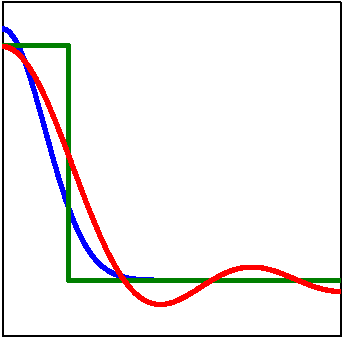
\includegraphics[width=\columnwidth]{pic/K} \linebreak{ $\Psi$}
		\end{column}
		\begin{column}{3.3cm}
		  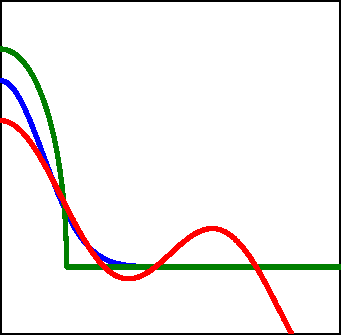
\includegraphics[width=\columnwidth]{pic/RK} \linebreak{ $\mathcal{R}\Psi$}
		\end{column}
		\begin{column}{3.3cm}
		  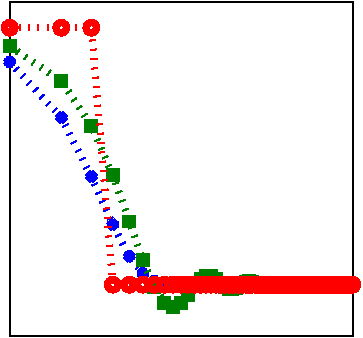
\includegraphics[width=\columnwidth]{pic/Fourier} \linebreak{ $\mathcal{F}\Psi$}
	  \end{column}
	\end{columns}
\end{center}

\end{frame}

\subsection*{Unimodal ODFs}

\begin{frame}[fragile]
  \frametitle{Defining Unimodal ODFs in \MTEX}

  \begin{columns}

    \begin{column}{8.5cm}

      Characteristics of an unimodal ODF:
      \begin{enumerate}
      \item crystal symmetry
      \item specimen symmetry
      \item modal orientation
      \item kernel function
      \end{enumerate}



\begin{lstlisting}
SS  = symmetry('orthorhombic')
CS  = symmetry('cubic')
o   = orientation('brass',CS,SS);
psi = kernel('von Mises Fisher',...
             'halfwidth',20*degree);
\end{lstlisting}

      \begin{actionenv}<1-| alert@1->
\begin{lstlisting}
odf = unimodalODF(o,CS,SS,psi)
\end{lstlisting}
    \end{actionenv}

\end{column}

    \begin{column}{3cm}
      \onslide<1->
      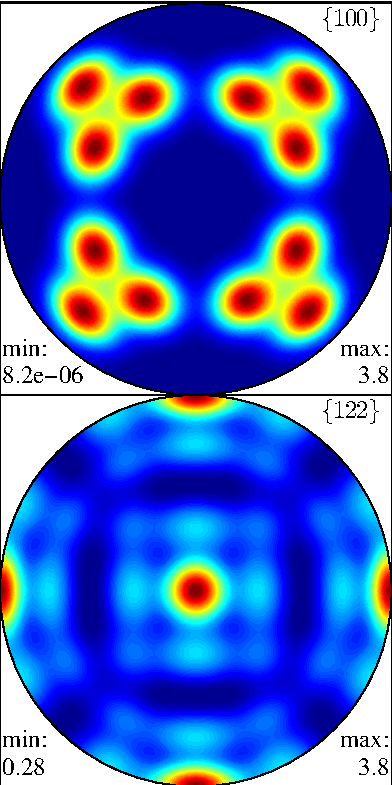
\includegraphics[width=3cm]{pic/unimodalODF}
    \end{column}
  \end{columns}

\end{frame}



\subsection*{Fibre ODFs}

\begin{frame}[fragile]
  \frametitle{Defining Fibre ODFs in \MTEX}

  \begin{columns}

    \begin{column}{8.5cm}

      Characteristics of a fibre ODFs:
      \begin{enumerate}
      \item crystal symmetry
      \item specimen symmetry
      \item crystal direction
      \item specimen direction
      \item kernel function
      \end{enumerate}


\begin{lstlisting}
SS = symmetry('triclinic')
CS = symmetry('hexagonal')
h = Miller(1,0,0,CS);
r = xvector;
psi = kernel('Abel Poisson',...
             'halfwidth',18*degree);
\end{lstlisting}

      \begin{actionenv}<1-| alert@1->
\begin{lstlisting}
odf = fibreODF(h,r,CS,SS,psi)
\end{lstlisting}
      \end{actionenv}

\end{column}

    \begin{column}{3cm}
      \onslide<1->
      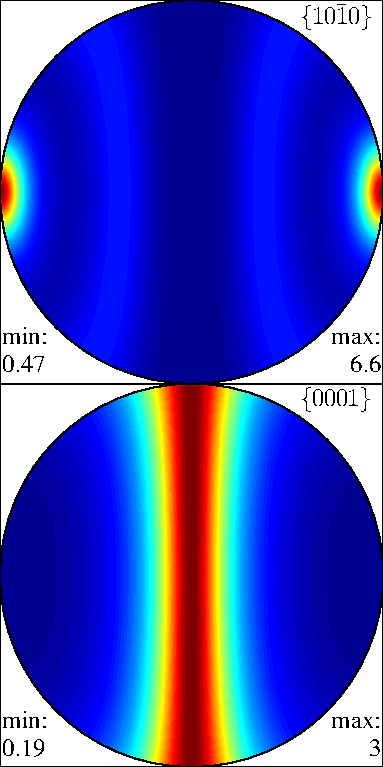
\includegraphics[width=3cm]{pic/fibreODF}
    \end{column}
  \end{columns}


\end{frame}


\subsection*{Bingham distributed ODFs}

\begin{frame}[fragile]
  \frametitle{Defining a Bingham distributed ODF}

\begin{lstlisting}
Kappa = [-10,-10,10,10]
A = quaternion(eye(4))
odf = BinghamODF(Kappa,A,CS,SS)
\end{lstlisting}

\end{frame}

\subsection*{Fourier ODFs}

\begin{frame}[fragile]
  \frametitle{Defining Uniform and  Fourier ODFs}

  The uniform ODF:
\begin{lstlisting}
SS = symmetry('triclinic')
CS = symmetry('hexagonal')
\end{lstlisting}

  \begin{actionenv}<1-| alert@1->
\begin{lstlisting}
odf = uniformODF(CS,SS)
\end{lstlisting}
  \end{actionenv}

  \begin{block}{Fourier expansion of an ODF}
    \begin{equation*}
      f(\mathbf g) = \sum_{l=0}^L \sum_{k,k'=-l}^l C_l^{k,k'} T_l^{k,k'}(\mathbf g)
    \end{equation*}
    \begin{equation*}
      C = [C_0,C_1^{-1,-1},C_1^{0,-1},C_1^{1,-1},\ldots,C_1^{1,1},C_2^{-2,-2},\ldots,C_L^{L,L}]
    \end{equation*}
  \end{block}
The Fourier ODF:
  \begin{actionenv}<1-| alert@1->
\begin{lstlisting}
odf = FourierODF(C,CS,SS)
\end{lstlisting}
  \end{actionenv}



\end{frame}

\subsection*{ODF Arithmetic}

\begin{frame}[fragile]
  \frametitle{ODF Arithmetic}


  \begin{columns}
    \begin{column}{6cm}

      Calculate with ODFs:
\begin{lstlisting}
odf1 = unimodalODF(...)
odf2 = fibreODF(...)
odf3 = uniformODF(CS,SS)

odf = 0.2*odf1 + 0.3*odf2
      + 0.5*odf3

\end{lstlisting}

  Rotate ODFs:
\begin{lstlisting}
rot = rotation(...
       'axis',xvector,...
       'angle',90*degree);
odf = rotate(odf,rot)
\end{lstlisting}


  Standard ODFs:
\begin{lstlisting}
odf = SantaFe;
\end{lstlisting}


\end{column}
\begin{column}{5cm}
  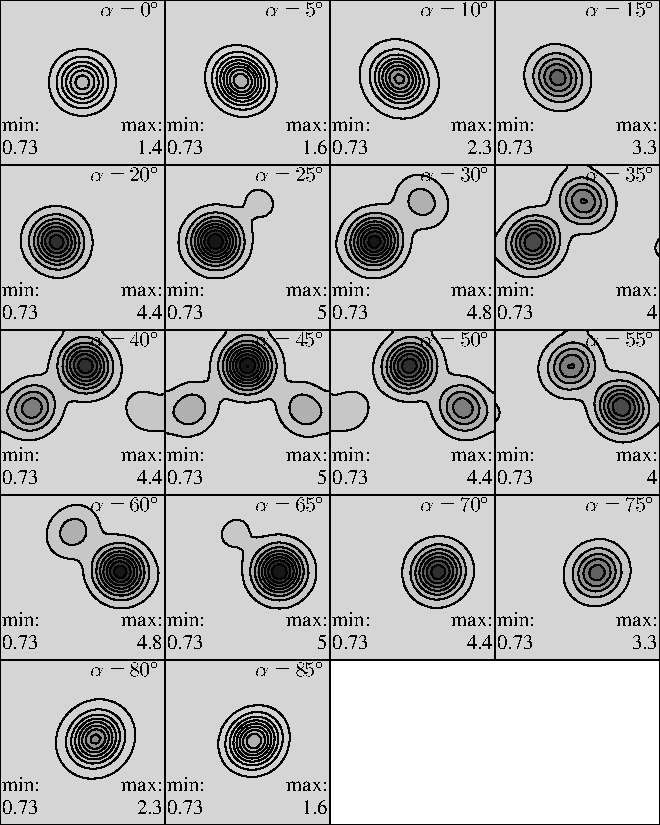
\includegraphics[width=5cm]{pic/santafeeh}
\end{column}
\end{columns}

\end{frame}

%%% Local Variables:
%%% mode: latex
%%% TeX-master: "main"
%%% End:
